
%\lipsum[101-120]
\section{The Building Game as a Mathematical Framework for Self-assembly}

The Building Game (BG) was first considered by Zlotnick~\cite{Zlotnick1994} as a model for the assembly of polyhedral viral capsids. In the model, a capsid is idealized as a polyhedron \poly\spc with each face treated as a subunit. Assembly proceeds from a singe face with a second face attached to the first along an edge. At each subsequent step of the process, an additional face is added along an edge of one of the already added faces. The process ends when all of \poly's face have been added resulting in a completed polyhedron.

A useful way to think about the Building game is as a sequential coloring process. Given a polyhedron with each face painted black, choose a face and paint it white. At each subsequent step, choose a black face that is adjacent to a white face ant paint it white. Repeat until all faces are white. Here the white faces symbolize the ones that are present at a given step of the assembly process.

\section{Formal Definition}
We formalize the Building Game in terms of the group action of the polyhedron \poly's roation group $\G$ acting on subsets of $F$, \poly's face set. 

\begin{mydef}
  A Building Game \textbf{state} $x \subset F$ is a non-empty subset of the faces of \poly such that the union of the faces without the vertices $\left(\cup_{f \in x}f\right) \setminus V$ is path connected. 
\end{mydef} 

%as a sequential graph labeling process. If we are interested in the BG of a polyhedron \poly, we represent \poly\spc by a graph $\PolyGraph = \left(F, E\right)$ whose nodes are the faces $F$ of \poly\spc and connections $E$ correspond to the pairs of faces sharing an edge of \poly. In this way, $\PolyGraph$ can be viewed as the polyhedral graph of \poly's dual polyhedron. 

%In Zlotnick's usage of the model, the labeling of $1$ or $0$ to each face would correspond to whether the face had been attached at some point up to the current step of the process. 
As pictured in figure~\ref{fig:OctaStates} an octahedron has 8 faces, 12 edges and 6 vertices. 

--More describing fig and what is and is not an intermediate.

%The corresponding $\PolyGraph$ representation is the octahedral graph with 6 vertices and 12 edges. In this example, the state represented labels three faces with a 1 and the others with 0. The embedded geometric interpretation shows three square faces connected along their edges.

\begin{figure}[ht]
  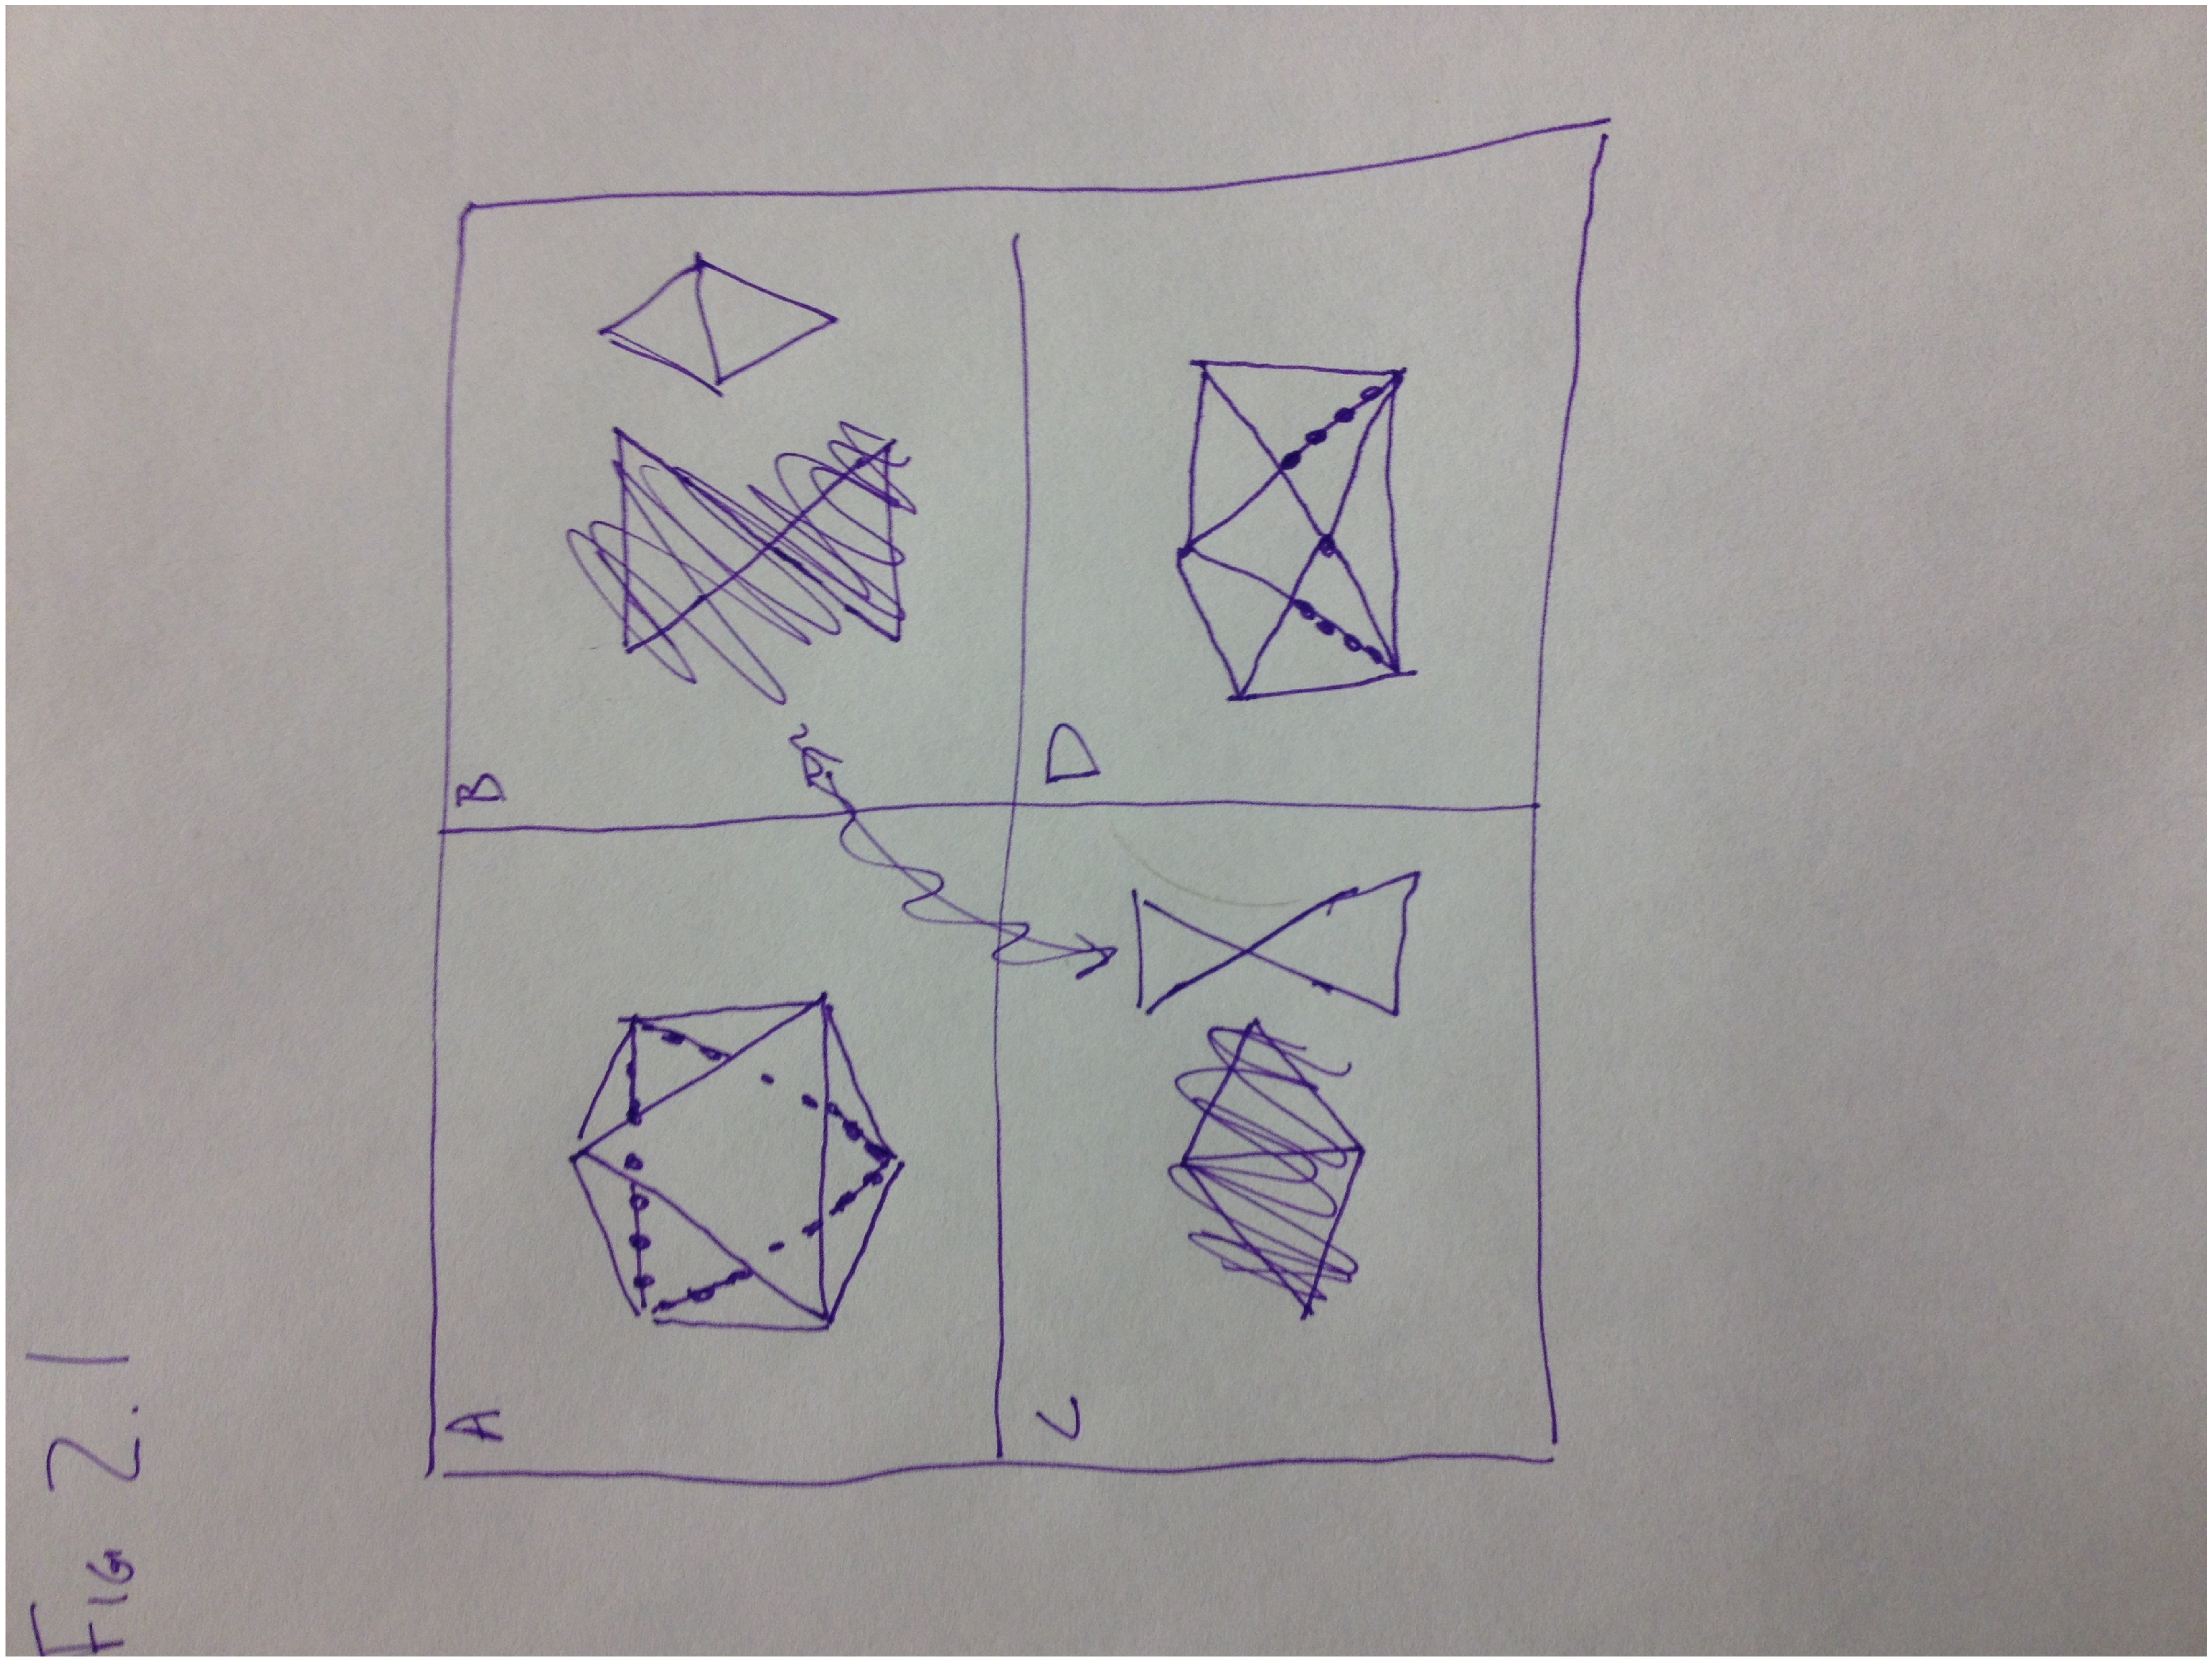
\includegraphics[scale=0.1, angle=0]{fig_2_1.eps}
\caption{The cube and its graph representation.}
\label{fig:OctaStates}
\end{figure}

%\begin{mydef}
%The Building Game \textbf{rotation group} $\G$ is the permutation group acting on $F$ that corresponds to \poly's rotational symmetry group.
%\end{mydef}

\begin{mydef}
The Building Game \textbf{stabilizer subgroup} for a state $x$ is the subgroup $\G_x \doteq \left\{g \in \G :g. x = x \right\} \leq \G$ permutations that fixes $x$.
\end{mydef}

\begin{mydef}
The \textbf{symmetry number} $r_x$ of a state $x$ is the order of its stabilizer subgroup $\left|\G_x\right|$.
\end{mydef}

As in Zlotnick, we group the states that are rotations of each other. 

\begin{mydef}
A Building Game \textbf{intermediate} $[x] \doteq \left\{g.x : g \in G\right\}$ is the orbit of the state $x$. 
\end{mydef}
Then, since the orbits of a group action form a partition on the set it acts on, each state belongs to a single intermediate and two states $x$ and $y$ are part of the same intermediate if there is a $g\in\G$ such that $y = g.x$. 


\begin{mythm}
If the states $x$ and $y$ are members of the same intermediate $\left[x\right]$, they have the same symmetry number and thus we defin the \textbf{symmetry number} of an intermediate $\left[x\right]$ as $r_x$.
\end{mythm}
\begin{proof}
Let $h \in G$ such that $y = h.x$. Since $G$ is normal to itself, we have $G = h^{-1}Gh = hGh^{-1}$.
\begin{align}
  r_x &= \left|\left\{g \in \G :g. x = x \right\}\right| \\
  &= \left|\left\{g \in h\G h^{-1} : g.x = x \right\}\right| \\
  &= \left|\left\{ h^{-1}gh \in \G : (h^{-1}gh).x = x \right\}\right| \\
  &= \left|\left\{ h^{-1}gh \in h^{-1}Gh : (h^{-1}gh).x = x \right\}\right| \\
  &= \left|\left\{ g \in G : (h^{-1}gh).x = x \right\}\right| \\
  &= \left|\left\{ g \in G : (gh).x = h.x \right\}\right| \\
  &= \left|\left\{ g \in G : g.y = y \right\}\right| \\
  &= r_y
\end{align}
\end{proof}


\begin{figure}[ht]
\caption{The eight states in a particular BG intermediate.}
\label{fig:CubeState}
\end{figure}

%For ease of exposition, we use the notational shorthand $\left(x\right)_m$ for $x\left(f_m\right)$ and $x = g.x'$ when $x(f_m) = x'(g.f_m)$ for every $f_m \in F(\mathscr{P})$. Additionally, we denote the intermediate satisfying $\left(x\right)_m = \colorA$ for all $f_m \in \faceset$ as $x^\colorAsm$ and similarly $x^\colorBsm$ is the intermediate with $\left(x\right)_m = \colorB$ for all $f_m \in \faceset$. The function counting the number of \colorB\spc faces an intermediate has is denoted $h\left(x\right) \doteq |\left\{f_m \in \faceset : \left(x\right)_m = \colorB\right\}|$.

\begin{mydef}
Two intermediates $x^j$ and $x^k$ are \textbf{connected} ($x^j \leftrightarrow x^k$) if $\left(x^j\right)_m = \left(x^k\right)_m$ for all $f_m \in \faceset$ except for exactly one face $f_n$ that has  $\left(x^j\right)_n \neq \left(x^k\right)_n$.
\end{mydef}
\begin{mydef}
A Building Game \textbf{pathway} is a sequence of intermediates $x^{p_0}, x^{p_1}, x^{p_2}, \dots, x^{p_N}$ such that $x^{p_0} = x^\colorAsm$, $x^{p_N} = x^\colorBsm$, $x^{p_i}$ is connected to $x^{p_{i+1}}$ and $h\left(x^{p_i}\right) = i$.
\end{mydef}

In this way it is useful to think of intermediates as connected if it is possible to color one face of the first intermediate to get the second and a pathway as a sequence of these connections between $x^\colorAsm$ and $x^\colorBsm$. Figure~\ref{fig:DodecBG} shows a Building Game pathway for the dodecahedron using Schlegel diagrams. The pathways has 13 intermediates since there must be exactly one intermediate $x^{p_i}$ satisfying $h\left(x^{p_i}\right) = i$ for each $i = 0,1,2,\dots,12$.

\begin{figure}[ht]
\caption{One Building Game pathway on the dodecahedron.}
\label{fig:DodecBG}
\end{figure}

With many pairs of connected intermediates, we organize these relations in a graph.

\begin{mydef}
The Building Game \textbf{state space} for a polyhedron \poly\spc is a graph in which the nodes are \poly's intermediates and a graph edge exists between two intermediates if and only if they are connected. 
\end{mydef}

When the intermediates are partitioned by their value of $h$, it is natural to arrange the state space as a tiered graph according to this partition. Figure~\ref{fig:CubeSS} shows the Building Game state space for the cube. As seen, each tier has intermediates with the same number of \colorB faces and connections thus exist with intermediates that are either in the tier directly above or below them. We can also see that there are three distinct pathways contained in the state space. 

\begin{figure}[ht]
\caption{The Building Game state space of the cube.}
\label{fig:CubeSS}    
\end{figure}

Interestingly, it is not the case that the recoloring of each face of \xj\spc results in a distinct intermediate. 
\begin{mydef}
The number of different faces $\left|\left\{f_m \in \faceset : x^j + e^m \in \left[x^k\right]\right\}\right|$ of \xj\spc that can be colored to form \xk\spc is called the \textbf{degeneracy number} \Sjk.
\end{mydef}
It is important to note that in general the degeneracy number is not symmetric, i.e. \Sjk$\neq$\Skj\spc for some connections \xj\spc$\leftrightarrow$\spc\xk\spc in the state space. Both figures~\ref{fig:DodecBG} and ~\ref{fig:DodecBG} show the forward and backward degeneracy numbers for each connection.

\subsection{Related Work}
--Like polyominos on polyhedra

\subsection{Applications}
--Viral capsid assembly

--Self-assembly of molecular cages

--Self assembly for manufacturing purposes
%~\cite{Endres2005}
\subsection{Paper Overview}
-- Summary of subsequent sections

Since the Building Game is a sequential process with several choices at each step, it is natural to consider it as a stochastic process. By putting a distribution on all possible faces that can be colored \colorB\spc at each step of the Building game, a distribution on the space of pathways is implicitly defined. Thus, for a choice of this transition rule, we can ask questions about the likelihood of the different pathways. 

--Math and graphical results about putting a distribution on pathways


\subsection{A Finite Geometric Result}

Since we define Building Game intermediates as rotationally unique from each other, it is useful to think about the problem in the context of $\mathscr{P}$'s rotational symmetry group $G \doteq G\left(\mathscr{P}\right)$ and group actions. For an intermediate $x^j$, the number of symmetries $r_j$ is the order of the stabilizer subgroup $G_{x^j} \doteq \left\{g \in G : g.x^j = x^j\right\}$ of $G$ that fixes $x^j$. Suppose $x^j$ and $x^k$ are connected in the state space and $\varphi$ is one of the $S_{jk}$ faces that, when added to $x^j$, forms $x^k$. We say $x^j + \varphi = x^k$. The degeneracy number $S_{jk}$ can then be expressed as the order of the orbit $\left(G_{x^j}\right).\varphi$ of $\varphi$ with respect to $x^j$'s stabilizer subgroup. Analogously, we define the reverse degeneracy number as $S_{kj} \doteq \left|\left(G_{x^k}\right).\varphi\right|$

\begin{mylem}
\label{lem:I}
For Building Game intermediates $x^j$ and $x^k$ connected in the state space and a face $f_m \in \faceset$ satisfying $x^j + e^m = x^k$, the stabilizer subgroup $G_{x^j,e^m}$ that fixes both $x^j$ and $e^m$ is the same stabilizer subgroup $G_{x^k,e^m}$ that fixes $x^k$ and $e^m$.
\end{mylem}
\begin{proof}
\begin{align}
G_{x^j,e^m} &\doteq \left\{g \in G | g.x^j = x^j, g.e^m = e^m \right\} \\
                &= \left\{g \in G | g.\left(x^k - e^m\right) = x^k - e^m, g.e^m = e^m \right\} \\
                &= \left\{g \in G | g.x^k = x^k, g.e^m = e^m \right\} \\
                &\doteq G_{x^k,e^m}
\end{align}
\end{proof}


\begin{mythm}
\label{thm:J}
For two Building Game intermediates $x^j$ and $x^k$ are connected in the BG state space, $r_kS_{jk} = r_jS_{kj}$.
\end{mythm}
\begin{proof}
Let $e^m$ be a face such that $x^k = x^j + e^m$. Then, by the orbit-stabilizer theorem, Lagrange's Theorem and lemma~\ref{lem:I} we have the following~\cite{Rotman1995}.
\begin{align}
\frac{r_j}{S_{jk}} &\doteq \frac{\left|G_{x^j}\right|}{\left|\left(G_{x^j}\right).e^m\right|} \\
                   &= \left[G_{x^j} : \left(G_{x^j}\right).e^m \right] \\
                   &= \left|G_{x^j,e^m}\right| \\
                   &= \left|G_{x^k,e^m}\right| \\
                   &= \left[G_{x^k} : \left(G_{x^k}\right).e^m \right] \\
                   &= \frac{\left|G_{x^k}\right|}{\left|\left(G_{x^k}\right).e^m\right|} \\
                   &\doteq \frac{r_k}{S_{kj}} 
\end{align}
The result $r_kS_{jk} = r_jS_{kj}$ follows.
\end{proof}


\section{Stochastic Modeling Results}

If we allow faces be changed both from \colorA\spc to \colorB\spc and from \colorB\spc to \colorA, the process consists of transitions from intermediate to intermediate along state space connections. By specifying a distribution on these transitions, it will induce a stationary measure on the state space.  

We define the Markov process $X_t$ by the transition rate matrix $Q$, with the heuristic that the rate of transition to an intermediate \xk from an intermediate \xk should be proportional to the number of faces of \xj that can be colored to reach the intermediate \xk. For this reason, we include the degeneracy number \Sjk\spc as a factor in the transition rate matrix. Furthermore, we model the process after and energetic model in which each intermediate has an energy and to transtion between intermediates, an energy barrier $E_{jk} = E_{kj}$ must be overcome. 
%\begin{align}
%\label{eq:TransitionProbability}
% P_{jk} = \frac{1}{z_j}S_{jk}\rh 
%\end{align}
\begin{align}
\label{eq:TransitionRate}
Q_{jk} &= S_{jk}e^{-\beta\left(E_{jk} - E_j\right)} \\
Q_{jj} &= -z_j \\
\end{align}
Here, $z_j \doteq \sum_{\ell: \ell \neq j} S_{j\ell}e^{-\beta\left(E_{j\ell} - E_j\right)}$ is the rate at which the process leaves \xj. 

\begin{mythm}
\label{thm:StatDist}
If the transition rate matrix $Q$ can be decomposed as $Q = DC$ where $D$ is diagonal with each entry of the diagonal positive and $C$ is a non-negative symmetric matrix with $C_{jk} > 0$ if and only if $x^j$ and $x^k$ are connected, then $X_t$ has the unique stationary distribution $\pi = \diag\left(D^{-1}\right)$.         
\end{mythm}
\begin{proof}
First, we show $Q$ and $\pi$ satisfy detailed balance.
\begin{align}
\pi_jQ_{jk} &= \left(\frac{1}{D_{jj}}\right)\left(D_{jj}C_{jk}\right) \\
&= C_{jk} \\
&= C_{kj} \\
&= \left(\frac{1}{D_{kk}}\right)\left(D_{kk}C_{kj}\right) \\
                    &= \pi_kQ_{kj}
\end{align}

-- Prove aperiodicity 
-- Prove positive reccurence

\end{proof}

In order to use theorem~\ref{thm:StatDist} to find the stationary distribution for the transition rule~\ref{eq:TransitionProbability}, we must be able to decompose the degeneracy number \Sjk\spc to fit the template of $\mathbf{C}$ and $\mathbf{D}$. In the following section we derive group theoretic identities to show that this is possible.

\subsection{Hitting Times}

\begin{align}
	\tau^{A}_{j} &\doteq \inf\left\{t \geq 0 : X_t \in A, X_0 = x^j\right\}
\end{align}

\begin{align}
	\nu^{A}_{j} &\doteq \inf\left\{n \geq 0 : Y_n \in A, Y_0 = x^j\right\}
\end{align}

For $j \not\in A$.
\begin{align}
	E\left[\tau^{A}_{j}\right] &= E\left[E\left[\tau^{A}_{j} | Y_1 \right]\right] \\
        &= E\left[ Exp\left(z_j\right) + \tau^{A}_{Y_1} \right] \\
        &=  \frac{1}{z_j} + E\left[\sum_{k}\tau^{A}_{Y_1}\mathbbm{1}_{Y_1 = k}\right] \\
        &=  \frac{1}{z_j} + \sum_{k: k\neq j}E\left[\tau^{A}_{k}\right] P\left(Y_1 = k\right) \\
        &=  \frac{1}{z_j}\left(1 + \sum_{k: k\neq j}q_{jk}E\left[\tau^{A}_{k}\right]\right)     \\
  \sum_{k}q_{jk}E\left[\tau^{A}_{k}\right] &= 1 \\
\end{align}

For $j \in A$.
\begin{align}
	E\left[\tau^{A}_{j}\right] &= 0 \\
\end{align}

As a linear system:
\begin{align}
	\left(\diag\left(\mathbbm{1}_A\right) - \diag\left(\mathbbm{1}_{A^c}\right)Q\right)E\left[\tau^{A}\right] =\mathbbm{1}_{A^c}\\
\end{align}


\begin{align}
\psi_j^A\left(t\right) &\doteq P\left(\tau^A_j \leq t\right) \\
\psi_j^A\left(0\right) &= \mathbbm{1}_{j\in A} \\
\psi_j^A\left(t\right) &= 0 \forall j \in A \\                       
\end{align}

For $j \not\in A$.

\begin{align}
\psi_j^A\left(t\right) &\doteq P\left(\tau^A_j \leq t\right) \\
                       &= \sum_k P\left(\tau^A_j \leq t | Y_1 = x^k\right) P\left(Y_1 = x^k\right) \\ 
                       &= \frac{1}{z_j}\sum_{k: k \neq j} q_{jk} P\left(Exp\left(z_j\right)\tau^A_j \leq t\right)  \\
                       &= \frac{1}{z_j}\sum_{k: k \neq j} q_{jk} \int^t_0 P\left(\tau^A_j \leq t - s\right) z_j e^{-z_j s} ds  \\
                       &= \sum_{k: k \neq j} q_{jk} \int^t_0\psi^A_k\left(t-s\right)e^{-z_j s} ds  \\
                       &= \sum_{k: k \neq j} q_{jk} \int^t_0\psi^A_k\left(r\right)e^{-z_j\left(t-r\right)} dr  \\
e^{z_jt}\psi^A_j\left(t\right) &= \sum_{k: k \neq j} q_{jk} \int^t_0 e^{z_jr}\psi^A_k\left(r\right) dr  \\
e^{z_jt}\frac{d\psi^A_j}{dt} + z_j e^{z_j t} \psi^A_j\left(t\right) &= \sum_{k: k \neq j} q_{jk} e^{z_jt}\psi^A_k\left(t\right)  \\
\frac{d\psi^A_j}{dt} &= \sum_{k} q_{jk} \psi^A_k\left(t\right) 
\end{align}

Combining both cases, we get the linear system and solution.

\begin{align}
        \frac{d\psi^A}{dt} &= \diag\left(\mathbbm{1}_{A^c}\right)Q\psi^A \\
        \psi^A\left(0\right) &= \mathbbm{1}_{A} \\
        \psi^A\left(t\right) &= e^{\diag\left(\mathbbm{1}_{A^c}\right)Qt} \mathbbm{1}_{A} \\ 
\end{align}

This is the solution for the CDF of the stopping time $\tau^A$, but we can also compute the PDF explicitly for $t > 0$.

\begin{align}
        p\left(\tau^A = t\right) &= \frac{d\psi^A}{dt} \\
        &= \diag\left(\mathbbm{1}_{A^c}\right)Q\psi^A
\end{align} 



\subsection{Stationarity}

\begin{mythm}
\label{thm:E}
The Markov process $X_t$ defined by the transition rate matrix $Q$ in equation~\ref{eq:TransitionRate} admits the unique stationary distribution $\frac{1}{zr_j}e^{-\beta E_j}$ where $z \doteq \sum_\ell \frac{1}{r_\ell}e^{-\beta E_\ell}$ is the partition function. 
\end{mythm}
\begin{proof}
We take $C_{jk} \doteq \frac{S_{jk}}{zr_j}e^{-\beta E_{jk}}$ and notice that it is symmetric by theorem~\ref{thm:J}. With $D_{jj} \doteq zr_je^{\beta E_j}$ we have our partition.  
\begin{align}
Q_{jk} &= S_{jk}e^{-\beta\left(E_{jk} - E_j\right)} \\
       &= \left(zr_je^{\beta E_j}\right) \left(\frac{S_{jk}}{zr_j}e^{-\beta E_{jk}}\right) \\
       &= D_{jj}C_{jk}   
\end{align}
Thus, by theorem~\ref{thm:StatDist},  $\pi_j = \frac{1}{D_{jj}} = \frac{1}{zr_j}e^{-\beta E_j}$.
\end{proof}

